\epigraph{\textit{It's a safe banking system, a sound banking system. Our regulators are on top of it. This is a very manageable situation.}}{––\textsc{Henry Paulson}, Former Secretary of the Treasury \\ \textit{Two months prior to Lehman Brothers' collapse.}}

%%%%%%%%%%%%%%%%%%%%%%%%%%%%%%%%%%%%%%%%%%%%%%%%%%%
%. 3 parts to the Background:
%.  - Historical/Regulatory Context
%.  - Literature Review
%.  - Mathematical Preliminaries
%%%%%%%%%%%%%%%%%%%%%%%%%%%%%%%%%%%%%%%%%%%%%%%%%%%

\section{Introduction}
This chapter provides some wider context to the project. It begins with a broad overview of interest rate derivative and cryptocurrency markets in general, including their history, current landscape, and regulatory regimes. We then review the established literature relating to interest rates, specifically those pertaining to interest rate models, and some more recent papers regarding the interest rate environment and associated products within the crypto sector. Finally, we look at some of the fundamental mathematical definitions and results that will be used extensively throughout the project. 

%%%%%%%%%%%%%%%%%%%%%%%%%%%%%%%%%%%%%%%%%%%%%%%%%%%
%%%%%%%%%%%%%%%% HISTORY / CONTEXT %%%%%%%%%%%%%%%%
%%%%%%%%%%%%%%%%%%%%%%%%%%%%%%%%%%%%%%%%%%%%%%%%%%%
\section{History \& Context}

\subsection{A Brief History of Interest Rate Derivatives}
It was 1981 when the World Bank entered into the first \textit{currency swap}. The comparatively low level of interest rates in Germany and Switzerland meant they were facing increasing demand from borrowers seeking loans denominated in Deutsche marks and Swiss francs respectively. Unfortunately, the governments of both countries had imposed limits on the amount the World Bank could borrow and by August 1981 those limits had been reached. As it happened the U.S. company IBM was looking to increase its dollar holdings, having already garnered a sizable amount of bonds issued in marks and francs, and as such IBM and the World Bank agreed to swap currencies. Thus, the swap market was born. 

It was not until 1985 that the World Bank entered into its first \textit{interest rate swap}, initiated at par, for which an agreement was made to pay a floating amount of U.S. dollar interest, based upon the three-month World Bank Treasury bill rate, and receive a fixed rate of U.S. dollar interest.

From this point the market for swaps grew rapidly as both currency and interest rate swaps meant that parties could access new, alternative sources of funding in a financially practical way. In addition, it allowed parties to actively consider their risk management by means of converting their liabilities, either into a more appropriate currency or a more appropriate structure of interest payments \citep{WorldBank_Ch2_1}.

As the size grew, so too did the number of interest rate derivative products. \textit{Basis rate swaps}, \textit{interest rate swaptions}, and \textit{caps} and \textit{floors} were just a few of those introduced, while exotic features were added to established contracts as the market saw an explosion in demand, and opportunities. The swiftness of their introduction was thanks, in large part, to the fact that such products are traded \textit{Over-the-Counter} (OTC)––that is, the contracts simply involved the two respective parties with no central exchange or clearing house acting as mediator. As a result, the level of transparency was low. 

For over thirty years the market continued to flourish, quickly becoming one of the largest and most active in the world. The Bank for International Settlements reported that in the first half of 2008, the notional principle outstanding for interest rate derivatives stood at just under \$503 \textit{trillion} \citep{BIS_Ch2_1}, dominating other OTC asset classes as shown in Figure \ref{fig:notionals}. However, the financial crisis brought the market squarely into focus for regulators. 

\begin{figure}[ht]
\begin{center}
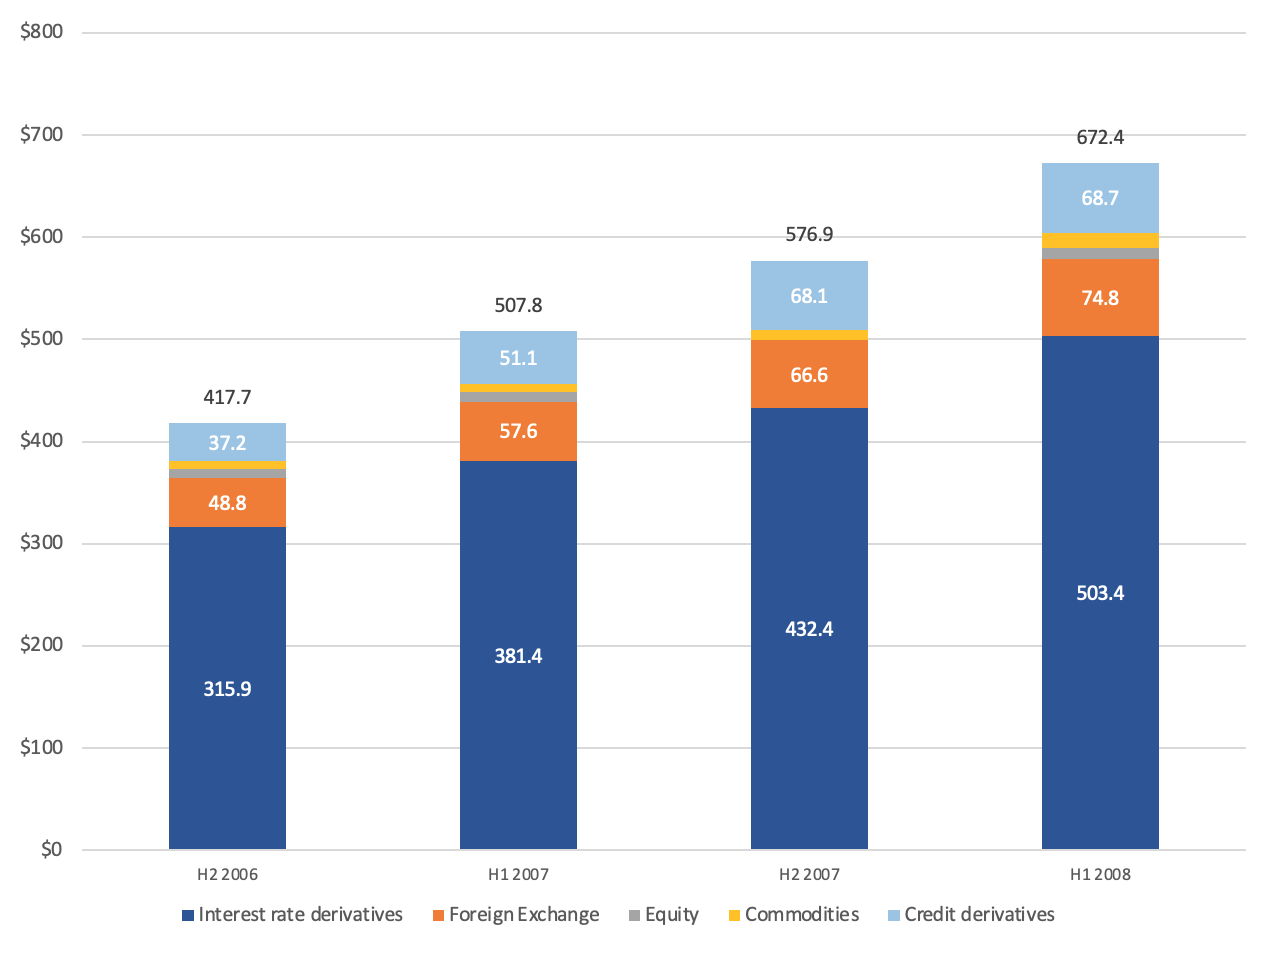
\includegraphics[width=0.95\textwidth]{Chapter_2/images/notionals.png}
\caption[OTC Derivatives Notional Outstanding USD (Trillions)]{The notional amounts outstanding across OTC derivatives markets for each half year from H1 2006 to H1 2008 in USD (trillions). We can clearly see the continuous growth over the period, and the domination of interest rate derivatives which had an outstanding notional greater than the sum of the other categories over the range. Data from \citep{BIS_Ch2_1}.}
\label{fig:notionals}
\end{center}
\end{figure}

\subsection{The Financial Crisis and the Current Landscape}
The financial crisis of 2007–2009 brought about a worldwide overhaul of financial regulations. In the U.S. the Dodd-Frank Wall Street Reform and Consumer Protection Act (``Dodd-Frank Act'') was passed, whilst the European Market Infrastructure Regulation (``EMIR'') was implemented in Europe––both of which were specifically designed to secure OTC derivatives markets in an effort to prevent another global collapse \citep{CFTC_Ch2_1}.

Despite these fundamental changes, the popularity of interest rate derivatives contracts did not waiver. In fact, the outstanding notional principle of the market peaked at \$587 trillion in 2011, although it has since stabilised to somewhere in the region of \$480–\$520 trillion in the last few years.

\FloatBarrier

What did change, however, was the logistics of the transactions and obligations of each party entering into such contracts. The primary objectives of the regulations can be summarised as follows \citep{EuroCom_Ch2_1}:
\begin{itemize}
    \item Introduction of central clearing for those OTC derivatives classed as standardised;
    \item Increased usage of an exchange or electronic platform for the trading of OTC derivatives classed as standardised;
    \item Increased capital requirements for organisations trading OTC derivatives contracts that are not centrally cleared, i.e. are not standardised;
    \item Increased minimum margin requirements for those OTC derivatives contracts that are not centrally cleared;
    \item Reporting of OTC derivatives trades to trade data repositories.
\end{itemize}

These factors are critical to well functioning and transparent OTC derivatives markets and there has been a great deal of investment by market participants into the underlying infrastructure. In addition, they will play an important role when we consider the extension of traditional interest rate derivatives to the world of cryptocurrencies so it is well worth examining the main points in more detail. 

\subsubsection{The Role of Central Clearing}
The introduction of central clearing for those contracts classed as standardised––essentially those that were the most liquid––was aimed at reducing the counterparty credit exposure of previous bilateral agreements. This meant, for certain interest rate derivatives, contracts \textit{must} involve a central counterparty (`CCP'). The CCP (normally a clearing house) would then act as `a buyer to every seller and a seller to every buyer' thereby reducing overall risk through netting\footnote{The general term used for the aggregation and subsequent simplification of multiple contractual obligations \citep{JSCC}.}. 

Initially, there were four contracts identified as standardised: \textit{fixed-for-floating swaps}, \textit{basis rate swaps}, \textit{overnight index swaps} (`OIS'), and \textit{Forward Rate Agreements} (`FRA'). In addition, only those contracts denominated in U.S. dollars, Pound Sterling, Euros, and Japanese Yen, were required to be cleared. This requirement has since been expanded to include a wider range of interest rate derivatives. 

Of course, the opportunity to reduce the level of risk involved in trades is certainly an attractive prospect. As such, in the first half of 2020, as much as 90.1\% of traded notional principle for interest rate derivatives was centrally cleared. The International Swaps and Derivatives Association (`ISDA') confirmed that market participants cleared a greater dollar amount than mandated under the current legislation \citep{ISDA_Ch2_1}. 

\subsubsection{Increased Capital Requirements}
For some contracts, however, the use of a CCP is either infeasible due to the bespoke nature of the specific contract or unwarranted due to the additional cost, after all, the services provided by the CCP are not free. In this scenario, the credit risk associated with a default by either party remains.

To combat this, the Basel Committee on Banking Standards (`BCBS') proposed a new BASEL III framework. This far reaching regulatory initiative included a section proposing new rules specifically relating to OTC derivatives by introducing a standardised methodology for calculating counterparty credit risk and credit valuation adjustments. This standardisation of approach resulted in market participants being obliged to hold increased capital reserves. BCBS reported that the amount of capital held by `Group 1'\footnote{BCBS defines \textit{Group 1} banks as those whose Tier 1 capital is greater than \euro 3 billion, in addition to those classified as `global systemically important' \citep{BCBS_Ch2_1}} banks more than doubled from \euro 2.3 trillion in 2011 to \euro 4.9 trillion in 2019 \citep{BCBS_Ch2_1}.

In a wider context, the BASEL III framework also had an impact on banks financial ratios. The \textit{net stable funding ratio}, \textit{liquidity coverage ratio}, and \textit{leverage ratio} all now have additional rules regarding the treatment of derivatives. For a detailed discussion of the impacts of BASEL III on financial institutions post-financial crisis see \cite{blundell2010thinking}, \cite{cosimano2011bank}, \cite{slovik2011macroeconomic}.

\subsubsection{Increased Margin Requirements}
In a similar manner, BCBS and the International Organisation of Securities Commissions (`IOSCO') produced a joint framework covering increased margin requirements for those contracts not involving a CCP \citep{IOSCO_Ch2_1}. This meant that both the \textit{initial margin} and \textit{variable margin} obligations were higher, again in an effort to reduce the credit exposure should one party experience default.

Like central clearing, posting greater margin protects both parties and is therefore mutually beneficial. As a result, an ISDA survey of those participants which were subject to the requirements under the first phase of implementation found that \$83 billion of initial margin not subject to the regulations was received. Furthermore, total initial margin levels for Phase 1 firms had more than doubled from \$130 billion in 2017 to \$286 billion in 2021 \citep{ISDA_Ch2_2}. 

\subsubsection{Transaction Reporting}
Since OTC derivatives pre-financial crisis were simply bilateral agreements, by definition, there was very little transparency of the underlying contracts. Regulators could investigate the transactions and portfolios of individual participants but could not easily obtain an aggregated view of the market. 

The requirement for derivatives transactions to be reported to Trade Repositories\footnote{In the U.S. interest rate derivatives transactions are reported to \textit{Swap Data Repositories} (SDR)––a diminutive of the more general term, Trade Repository.}, which would be registered and supervised by national competent authorities, meant that regulators now had improved visibility, and therefore sufficient oversight, of OTC markets.

The local regulatory regimes (EMIR for Europe, Dodd-Frank for the U.S.) set forth the mandatory data that must be provided to Trade Repositories. The interested reader is referred to the websites of regulatory authorities for more information (see the Financial Conduct Authority post-EU Withdrawal \citep{FCA_Ch2_1}; the European Securities \& Markets Authority \citep{ESMA_Ch2_1}; and the Securities \& Exchange Commission \citep{SEC_Ch2_1}).

\subsection{Market Participants}
The history and current landscape of interest rate derivatives provides important context, however, it does nothing to answer the question: who are the major market participants? In general, derivatives markets can be broadly considered to have four distinct, but invariably interlinked, participants: Hedgers, Speculators, Systematic Traders, and Arbitrageurs. For more detail, see \cite{chernenko2011two}, \cite{chui2012derivatives}, \cite{stankovska2017global}.

\subsubsection*{Hedgers}
Participants classed as \textit{hedgers} are those who wish to reduce their risk. They do so by entering into appropriate derivatives contracts that reduce the uncertainty of future prices and protect against any future market volatility. 

In general, for companies entering derivatives markets as hedgers, such activities do not form part of their core business. Whilst their main objective may be to reduce uncertainty, they still fundamentally require the assets to perform business functions and as such are likely to have an asymmetrical approach to losses. Consider the aviation industry. Taking a loss on a delivery of jet fuel is clearly less critical than the necessity of having the jet fuel available to fly planes.

\subsubsection*{Speculators}
Hedging can be considered a common sense strategy for those companies that require derivatives products and their underlying securities in order for their business to function. Yet it should be obvious that it is not only those companies which partake in such transactions. Generally speaking, those that are simply making predictions about the future, and seeking to profit should their view be correct, are called \textit{speculators}. In contrast to hedgers, this forms the core business of speculators. 

%Stobart Capital believes they have constructed a model that can predict where the FTSE100 will be at the end of each calendar year and as such is looking to profit. The current political landscape does not look good, hence, the model predicts with a high degree of confidence that the FTSE100 will be well below its current level, and thus Stobart Capital decides to short FTSE100 futures contracts. At the end of the year the index has fallen considerably and the futures contracts provide a large payoff.

The key point under these circumstances is that the motivation to enter the derivatives market is driven by profit seeking opportunities rather than as a risk mitigation strategy. A company may hold a strong belief, but does not truly know––that is, they are \textit{speculating}––how the price of an underlying asset will develop over the time horizon. If the market moves in the opposite direction, significant losses can quickly occur.

\subsubsection*{Systematic Traders}
\textit{Systematic trading} relies on a combination of technology, algorithms, and market signals. By setting clear, well defined strategies based on empirical data analysis and backtesting, systematic traders aim to remove any behavioral characteristics associated with the humans involved. The algorithmic implementation has the additional benefits of executing orders, taking profits, cutting losses, and managing risks in real time without the need for constant oversight. 

In practice this requires significant initial investments in technology and data in order to perform the necessary analyses to identify appropriate signals and markets––as well as employees with knowledge of mathematics, computer science, economics, and finance––which can act as a barrier to entry. Therefore systematic trading lends itself to hedge funds, and large global financial institutions.

\subsubsection*{Arbitrageurs}
Financial markets exist across the world, with a security sometimes being traded in multiple locations. For instance, a share may be traded on both the London and New York Stock Exchanges. Should those markets make a mistake and display different prices for the same underlying share (accounting for exchange rates), it would be possible for a party to make riskless profit by buying on the cheaper exchange and instantly selling on the more expensive exchange until the mispricing was corrected. Those participants that look for such opportunities are called \textit{arbitrageurs} and play a vital role in the efficient functioning of global financial markets. 

In practice, if and when such mispricings occur they may only exist for milliseconds. To take advantage, companies pursuing arbitrage strategies usually invest heavily into technology that can handle such low latencies, with companies even relocating offices closer to exchanges in an effort to receive information marginally faster than competitors. These barriers to entry tend to limit participation to specialist firms. 

\subsection{The LIBOR Transition}
Naturally, interest rate derivatives rely on an interest (or reference) rate and for much of their history this was the \textit{London Interbank Offer Rate} (`LIBOR'). LIBOR was essentially the rate at which large, global banks would lend to each other, and was calculated on a daily basis for five currencies and seven maturities. This benchmark was then used extensively throughout financial markets involving interest rates.

By virtue of its definition, LIBOR itself was not impacted by the financial crisis and changing regulations––although that is not to say the \textit{level} of LIBOR was not impacted, it was, in fact, much higher during this period as one would expect. However, LIBOR is not without its own historical issues. In 2008, critics suggested that banks could be understating their submissions, thereby giving the impression that other banks could borrow at a rate cheaper than they could in reality. This led to Mervyn King, former Governor of the Bank of England, to say that LIBOR was ``\textit{the rate at which banks didn't lend to each other}'' \citep{TSC_Ch2_1}. Furthermore, in 2012 it was discovered that companies had been attempting to manipulate LIBOR through their submissions in what later became known as the \textit{LIBOR scandal}. Barclays, for instance, was fined a total of \$435 million for its role \citep{Libor_Ch2_1}. 

More recently, however, a new regulatory regime was established that sought to transition away from LIBOR and towards alternative \textit{risk free rates} instead. The aim of this transition was to produce a rate that was based on historical data, rather than being forward-looking, which would make the benchmark more robust. As a result, the new benchmarks are now locally administered and overseen, that is, each jurisdiction will govern their own rate. 

At the end of 2021, LIBOR ceased to be applicable and was replaced by the \textit{Sterling Overnight Index Average} (`SONIA') in the U.K.; the \textit{Secured Overnight Financing Rate} (`SOFR') in the U.S.; and the European Short Term Rate (`ESTER') in Europe––with the exception of certain U.S. dollar denominated maturities which will continue for slightly longer \citep{FCA_Ch2_2}. 

\subsection{A Brief History of Cryptocurrencies}
Despite its prolific rise over the past decade, the origins of cryptocurrencies can be traced back to the 1980's when an American computer scientist by the name of David Chaum created an electronic, cryptographic currency called electronic cash (\textit{e-cash}) \citep{chaum1983blind}. In fact, a few years before its creation, a dissertation by the same author provided what is considered to be the first implementation of the blockchain concept \citep{chaum1979computer}.

E-cash did not survive, however, but the idea had been firmly established. In the late 1990's, \textit{B-Money} \citep{Bmoney1998} and \textit{Bit Gold} \citep{BitGold1998} were attempts to develop digital currencies utilising encrypted ledger technology but never fully materialised. Then, in 2008, Satoshi Nakamoto (a presumed pseudonym) published a paper entitled \textit{Bitcoin: A peer-to-peer electronic cash system} \citep{nakamoto2008bitcoin}. The following year Bitcoin was made open-source, and still remains the flagship cryptocurrency to this day.

Bitcoin itself has a rich history from those early days to the present, however, this project is focused more generally on the concept of cryptocurrencies and derivatives thereof. As such, we will not go into any further detail. The interested reader is referred to \cite{bohme2015bitcoin} and \cite{zohar2015bitcoin} for more information regarding the Bitcoin concept, or \cite{urquhart2016inefficiency} for some of the challenges it faces. 

\subsection{The Current Landscape, Products \& Regulatory Oversight}
With increasing reliance on digital technologies across all aspects of our lives, it seems impossible to ignore the world of cryptocurrencies. After all, \cite{bloomberg} reported that the total market cap at the end of 2021 was over \$3 trillion. Since Bitcoin's successful introduction, the number of available tokens has exploded and \cite{CNBC} reported there are approximately 19,000 cryptocurrencies in existence. This is in part due to the ease with which one can create new tokens by simply launching on the desired existing framework. Naturally, there are drastic differences in both the value, maturity, and legitimacy of these digital currencies, and the vast majority of newly issued coins (through a so called Initial Coin Offering, or `ICO') fail rapidly \citep{blaseg2018dynamics}. However, these facts do characterise the recent popularity and increased attention being paid to the sector. Of course, as popularity increases so too does the demand for products. 

Despite their decentralised nature, cryptocurrencies are still conceptually similar to currencies, and the world of derivatives can easily be extended from their traditional counterparts. As a result, several crypto exchanges have appeared offering two major benefits: firstly, reducing the barriers to entry for those investors interested in trading cryptocurrencies but who lack the technical expertise (or resources) to participate in the underlying computational activities; and secondly, extending the product offering for major cryptocurrencies through the likes of derivatives. In fact, the introduction of derivatives caused a jump in value across the sector and was seen as a major statement regarding the seriousness of crypto markets \citep{Gemeni}.

As a result, crypto futures and options are now available. These contracts behave largely the same as their traditional counterparts, with features like initial and variable margin requirements, and both delivery and perpetual contracts. However, there are additional non-technical features such as \textit{Leaderboards} and \textit{Battle}––which pits two traders head-to-head to see who is the most profitable over a set time period. These are designed to enhance the experience of traders through the so called ``\textit{gamification of cryptocurrency trading}" \citep{binance}.

These changes have not gone unnoticed by regulators and the sector has been placed under the spotlight in the last couple of years. However, cryptocurrencies present a challenging situation for regulators worldwide as they fall right on the border of the regulatory perimeter. The UK Financial Regulator has stated that ``\textit{cryptoassets are not underpinned by any currency or other asset and are not considered to be a currency or money}" \citep{FCA_Ch2_3}. This means that the only oversight provided to cryptocurrencies themselves (e.g. Bitcoin) is for money laundering purposes. On the other hand, they have also stated that ``\textit{cryptocurrency derivatives are capable of being financial instruments under MiFID II}" \citep{FCA_Ch2_4}, thereby requiring compliance with the authorisation and regulation in the same manner as for traditional financial derivatives––this includes futures and options contracts. 

The onus, though, is on the firm themselves to seek out and establish whether their products and services fall under this regime. Consequently, the number of scams has been high, but even legitimate firm collapses have left consumers with significant losses. Of course, where the responsibility lies in such cases and the extent to which regulations should be enforced is left to the opinion of the reader. Nevertheless, it is expected that the sector will continue to receive increasing regulatory attention over the coming years.


%%%%%%%%%%%%%%%%%%%%%%%%%%%%%%%%%%%%%%%%%%%%%%%%%%%
%%%%%%%%%%%%%%%%%%% LIT REVIEW  %%%%%%%%%%%%%%%%%%%
%%%%%%%%%%%%%%%%%%%%%%%%%%%%%%%%%%%%%%%%%%%%%%%%%%%

\section{Literature Review}
Much of the literature regarding interest rates and their respective derivatives has been established for some time since the flurry of proposals between 1970 and 2000. For the most part the proposals could be classified as short rate models, but there were some alternative ideas as well. For an excellent and incredibly detailed treatment of the world of interest rates and their derivatives, the reader is referred to \cite{brigo2001interest}.

Short rate models are built on the instantaneous \textit{spot rate} being the underlying variable for the stochastic process, thereby allowing interest rate derivatives to be priced under an appropriate risk-neutral measure. There are numerous famous models of this type including simpler one-factor models such as that of \cite{vasicek1977equilibrium} who proposed a mean-reverting stochastic process (although, it was simply a specific case of the Ornstein-Uhlenbeck process from Physics). This model was criticised for allowing negative interest rates, however, the longstanding belief that interest rates could not turn negative has since been overturned.

To account for this, Cox, Ingersoll, and Ross proposed a modified stochastic process \citep{cox1985theory} which included the square root of the instantaneous interest rate in the diffusion term preventing non-zero rates and, provided the Feller Condition was satisfied, would not become absorbed at zero either. Since then, numerous other models have been proposed, each with slight modifications aimed at better capturing the term structure including that of \cite{ho1986term}, \cite{hull1993one}, \cite{black1991bond}, and Black, Derman, and Toy \citep{black1990one}. There have also been two-factor models proposed, such as that of \cite{longstaff1992interest} which separates the behaviour of short term and long term interest rate movements and produces a linear combination of the two. 

One of the alternatives to short rate models, were those developed under the Heath-Jarrow-Morton (HJM) framework \citep{heath1992bond}. Such models are based on the instantaneous \textit{forward rate} and are aimed at describing the full dynamics of the forward curve as opposed to simply a single point on the curve, as with short rate models. Similarly, another alternative was a new class called the LIBOR market model, or Brace-Gatarek-Museila (BGM) model \citep{brace1997market}, which proposed modelling a \textit{set of forward rates}. This was a significant change when pricing interest rate derivatives as it now meant using an appropriate \textit{forward} measure.

Of course, the natural question is: which interest rate term structure model should be used? In truth, the nature of the derivatives contract itself largely dictates the model with more complicated, exotic contracts restricting the choice. For instance, the LIBOR market model is well suited to Bermudan swaptions, while plain vanilla swaptions can be priced under the simpler \cite{black1976pricing} model.

Interestingly, however, the focus of our project––pricing interest rate swaps––does not require the interest rate model. As a result, the literature relating to the topic is largely homogeneous, that is, ignoring notational differences the method to price interest rate swaps is standardised, clearly understood, and widely accepted in practice. Hence, we have used \cite{brigo2001interest}, \cite{sadr2009interest}, \cite{flavell2012swaps}, \cite{wilmott2013paul}, \cite{veronesi2016handbook} for reference throughout this project. 

Since crypto is still a relatively immature sector, there is little to no literature discussing crypto interest rate swaps. In fact, one of the more pressing, fundamental challenges is what do we mean by the concept of `interest' in the crypto market. Several papers have been published over the last few years proposing new ideas, models, and mathematical frameworks aimed at addressing this current gap.

A paper put forth by \cite{brody2020theory} proposed a model for the term structure of interest rates in the world of cryptocurrencies, in which the typical numeraire––the money market account––does not exist. This model builds on the extensive literature regarding the short rate, some of which we have just mentioned, and establishes a non-trivial `no interest' environment, that is, the spot rate is zero for all time and yet the term structure is non-zero and we can construct yield curves. This will be examined in greater detail in Chapter 4.

The paper by \cite{kaneko2019management} suggests a model based on Unspent Transaction Output (``UTXO") which adds a second layer to an underlying blockchain technology. This second layer extends the transaction data captured on the existing blockchain to include another program capable of managing the concept of interest. To do so, their model proposes issuance of two, equal and offsetting transactions––one acting as the loan itself, which would subsequently be transferred to the borrower, whilst the other would play the dual role of maintaining the `\textit{currency conservation law}' and a claim for the loan amount against the borrower. 

The strength of the model lies in its ability to account for both fixed and floating rates as follows. For floating rates of interest, a further issuance of two equal and offsetting transactions in the amount of the interest, determined precisely at (or before) the point of issuance. This could then be repeated as many times as required, with each transaction being stored and completely verifiable by other participants on the \textit{secondary layer of the blockchain}. Fixed rates of interest are managed once again by the issuance of two equal and offsetting transactions, however, this time they are all issued at initiation and rely on programs that implement a suspension period before becoming active. 

Unfortunately, the model is not free of challenges. Mainly, the issuance and subsequent closure of any loans requires what they classify as a \textit{Bank authority}. This introduces the idea of specific roles performing specific functions with respect to the loan and subsequent handling––for instance, they state that only such Bank authorities should have the ability to close the loan. This, in turn, greatly increases the complexity of the model both from a conceptual and implementation perspective. 

%%%%%%%%%%%%%%%%%%%%%%%%%%%%%%%%%%%%%%%%%%%%%%%%%%%
%%%%%%%%%%%%%%% MATH PRELIMINARIES %%%%%%%%%%%%%%%%
%%%%%%%%%%%%%%%%%%%%%%%%%%%%%%%%%%%%%%%%%%%%%%%%%%%

\section{Mathematical Preliminaries}

We now introduce the mathematical notation used throughout this project and present some fundamental terminology along with their precise definition. 

\subsection{Discount Factors}
The world of fixed income is synonymous with the concept of the \textit{time value of money}. The idea that a specific amount of money received in the future must have some present value. Since the amount of money is arbitrary, we can consider the case of receiving \$1 at some time in the future. We will define the \textit{discount factor} to be the present value of that \$1.

Let us formalise this concept, following the same notation as that of \cite{wilmott2013paul} and \cite{veronesi2016handbook}.

\begin{definition}[Discount factor]
\label{disc_fact}
    Let $t_0 = 0$ be today, and $t_i$ denote some time in the future, that is, $0 = t_0 < t_i $. Then we will define the \textit{discount factor} to be the present value of \$1 received at time $t_i$ and denote this as $Z(0, t_i)$.
\end{definition}

We can think of $Z(0,t_i)$ as the price today of a zero coupon bond. Assuming interest rates are non-negative (which is usually, but certainly not always, the case), we can construct a downward sloping curve of discount factors called the \textit{discount curve}.

\vspace{0.75cm}

\begin{figure}[ht]
\begin{center}
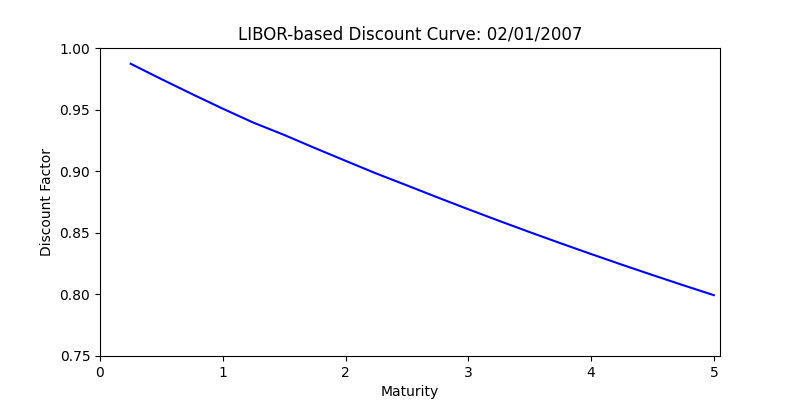
\includegraphics[width=0.95\textwidth]{Chapter_2/images/ch2_discount_factors.png}
\caption[LIBOR-based Discount Curve on 02/01/2007]{An example of a discount curve out to five years constructed from LIBOR-based instruments on 02/01/2007. Note the decreasing nature of the curve, indicating that receiving a hypothetical \$1 further into the future has a lower present value today. Reproduced from \cite{veronesi2016handbook}. Source data from Bloomberg.}
\label{fig:disc_curve}
\end{center}
\end{figure}

\subsection{Spot Rates}

Our discount factors give us the present value of \$1 received at some time in the future. Suppose we now flip the problem and instead of thinking about the present value of \$1, we consider what \$1 will be worth at some future point. To answer this question, we can use the concept of \textit{spot rates} (also called \textit{zero rates}), although we must take care with the compounding frequency. In what follows we standardise the notation of \cite{sadr2009interest} and \cite{brigo2001interest}. Let us first introduce the simplest case: the money market account.

\begin{definition}[Money market account]
\label{money_market}
    Let $B(t)$ be the value of a money market account at some point, $t$, in the future. We will assume an initial deposit of $B_0$, that is $B(0) = B_0$. Further, assume a \textit{constant, continuously compounded annual return}, $r$. Then the value of the money market account evolves according to the following ordinary differential equation,
    \begin{equation}
        \frac{dB(t)}{dt} = r B(t)
    \end{equation}
    which has solution
    \begin{equation}
        B(t) = B_0 e^{rt}.
    \end{equation}
\end{definition}
Our assumption of a single constant continuous rate, $r$, makes this calculation almost trivial. However, as we shall see in Chapter 4, when developing traditional interest rate models using the money market numeraire, we relax the constraint and assume the rate, $r_s$, is a positive function of time for $0 < s < t$. This leads to the more general expression,
\begin{equation}
    B_s = \exp \left( \int_0^s r_u du \right).
\end{equation}

Our money market account is, in fact, a direct relation between present and future values. In practice, rather than having one single continuous rate, we may have multiple rates (quoted on an annualised basis) which differ depending on the time period––consider fixed rate savings accounts which offer greater returns the longer the initial deposit is locked up.

\begin{definition}[Continuous zero/spot rate]
\label{cont_zero_rate}
    Let $r_c(t_i)$ be the \textit{continuously compounded annual return} of \$1 invested today until a future time, $t_i$ (in years). Then we will refer to $r_c(t_i)$ as the \textit{continuous spot rate} which relates present and future values via
    \begin{equation}
        FV =  PV e^{r_c(t_i) t_i}.
    \end{equation}
\end{definition} 
Note that the spot rate, $r_c(t_i)$, depends on the time as discussed.

Assuming a present value of unit currency to simplify notation, we can relate discount factors and spot rates via
\begin{equation}
    \frac{1}{Z(0,t_i)} = e^{r_c(t_i) t_i},
\end{equation}
which upon rearranging gives
\begin{equation}
    r_{c}(t_i) = -\frac{1}{t_i} \ln Z(0,t_i).
\end{equation}

The treatment of the discrete case is analogous.

\begin{definition}[Discrete spot rate]
\label{zero_rate}
    Let $r_d(t_i)$ be the \textit{discretely compounded annualised return} of \$1 invested today until a future time, $t_i$ (in years). In addition, suppose the return is compounded a discrete number, say $k$, times per year. Thus, $kt_i$ represents the total number of compounded periods. Then the return $r_d(t_i)$ is called the \textit{discrete spot rate} which relates present and future values via
    \begin{equation}
        FV =  PV \left(1 + \frac{r_d(t_i)}{k} \right)^{k t_i}.
    \end{equation}
\end{definition}

Once again, we can see the intrinsically linked nature of discount factors and spot rates via
\begin{equation}
    \frac{1}{Z(0,t_i)} = \left(1 + \frac{r_d(t_i)}{k} \right)^{k t_i}.
\end{equation}

Increasing the number of periods, $k$, per year and taking the limit we find
\begin{align}
    \frac{1}{Z(0,t_i)} &= \lim_{k \rightarrow \infty} \left[ \left(1 + \frac{r_d(t_i)}{k} \right)^{k} \right]^{t_i} \\
    &= \left[ \lim_{k \rightarrow \infty} \left(1 + \frac{r_d(t_i)}{k} \right)^{k} \right]^{t_i}.
\end{align}
Noting that the inner limit is precisely the definition of the exponential, we arrive at the continuous result above. 

This ability to transition between discrete and continuous spot rates is an important result and will be utilised when we consider curve construction in Chapter 3. To make the relation explicit we can equate our two methods to compute future values,
\begin{align}
    PV e^{r_c(t_i) t_i} &= PV \left(1 + \frac{r_d(t_i)}{k} \right)^{k t_i} \\
    e^{r_c(t_i) t_i} &= \left(1 + \frac{r_d(t_i)}{k} \right)^{k t_i} \\
    r_c(t_i) &= k \log \left(1 + \frac{r_d(t_i)}{k} \right).
\end{align}
Alternatively, using the fact that the number of compounding periods per year is inversely related to the time in years, that is $t_i = \frac{1}{k}$, we obtain the equivalent expression \citep{banque_canada}
\begin{equation}
    r_c(t_i) = \frac{1}{t_i} \ln ( 1 + r_d(t_i) t_i).
\end{equation}
Throughout this project we will use the subscripts, $d$ and $c$, to indicate whether the interest rate is discretely or continuously compounded.

Given a series of spot rates we can construct the \textit{spot curve}. 

\vspace{0.75cm}

\begin{figure}[ht]
\begin{center}
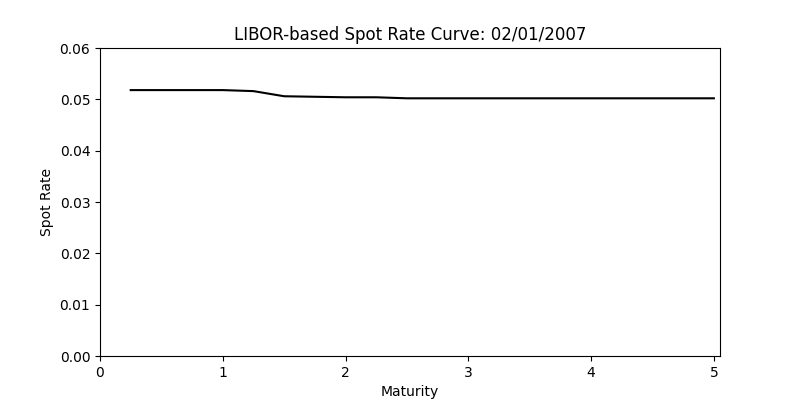
\includegraphics[width=0.95\textwidth]{Chapter_2/images/ch2_spot_rates.png}
\caption[LIBOR-based Spot Curve on 02/01/2007]{An example of a spot curve out to five years constructed from LIBOR-based instruments on 02/01/2007. The results in this graph can be constructed from the data given in Figure \ref{fig:disc_curve} and vice versa. Reproduced from \cite{veronesi2016handbook}. Source data from Bloomberg.}
\label{fig:spot_curve}
\end{center}
\end{figure}

\subsection{Forward Rates}

The spot curve is a useful tool for examining rates today, however, it gives little information about rates in the future. For that, we must look at \textit{forward rates}.

Forward rates establish a \textit{fixed} rate of interest for a specified time period \textit{starting at some point in the future}. That is, in order to understand a forward rate we need, not one, but two times: the start of the period and the end. We will follow the notation of \cite{veronesi2016handbook} and denote this as $f(0,t_{i-1}, t_i)$. As with spot rates, there is also the compounding frequency to consider.

A natural question arises: how do we determine a rate of interest for a period of time in the future? After all, we can only observe today's spot rates. Fortunately, we can rely on the concept of `no arbitrage' to establish the appropriate forward rate.

Consider two future times, $0 < t_1 < t_2$. From either the discrete or continuous definition of spot rates, we know that the amount received at time $t_1$ is $1/Z(0,t_1)$ and likewise at time $t_2$ is $1/Z(0,t_2)$. 

Then by the principle of no arbitrage we must have that investing at the spot rate associated with time $t_1$ and then reinvesting for the period $[t_1, t_2]$ should earn no more or less than simply investing at the rate associated with time $t_2$. In mathematical terms, we have

\begin{equation}
    \frac{1}{Z(0, t_1)} \times (1 + f(0,t_1,t_2)) = \frac{1}{Z(0, t_2)}.
\end{equation}

Rearranging gives rise to the following definition.

\begin{definition}[Discrete forward rate]
\label{fwd_rate}
    Let $f_d(0,t_{i-1},t_i)$ be the \textit{annualised forward rate} between $t_{i-1}$ and $t_i$ and let $Z(0,t_{i-1})$, $Z(0,t_i)$ be the associated discount factors. Then we can compute the discretely compounded forward rates as
    \begin{equation}
        f_d(0, t_{i-1}, t_i) = \frac{\frac{Z(0, t_{i-1})}{Z(0,t_i)} - 1}{t_i - t_{i-1}}.
    \end{equation}
\end{definition}

\begin{definition}[Continuous forward rate]
\label{cont_fwd_rate}
    As with the spot rate, we can compute the continuously compounded forward rate.
    \begin{equation}
        f_{c}(0,t_{i-1}, t_i) = \frac{\ln [ Z(0,t_{i-1}) / Z(0,t_i)]}{t_i - t_{i-1}}.
    \end{equation}
\end{definition}

Note that by starting our forward period today in definitions \ref{fwd_rate} and \ref{cont_fwd_rate} we simply arrive at the spot rate. Once again, we can construct the \textit{forward curve} given knowledge of the appropriate forward rates.

\vspace{0.75cm}

\begin{figure}[ht]
\begin{center}
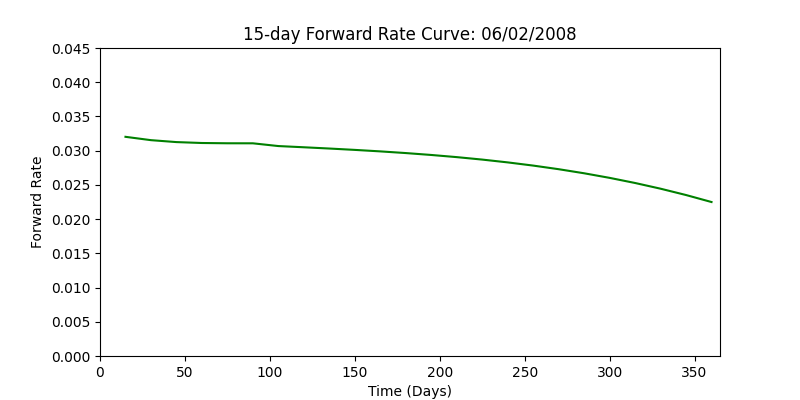
\includegraphics[width=0.95\textwidth]{Chapter_2/images/ch2_fwd_rates.png}
\caption[15-day Forward Curve on 06/02/2008]{An example of a 15-day forward rate curve over a one year horizon on 06/02/2008. Constructed from the data provided in \cite{flavell2012swaps}.}
\label{fig:fwd_curve}
\end{center}
\end{figure}

\newpage

Overall, we can see from Figure \ref{fig:linked_rates} the linked nature of the discount factors, spot rates, and forward rates. With knowledge of one, we can compute the others giving us a full picture of the current interest rate environment. We can consider discount factors as `pure', by which we mean the choice of compounding does not affect them. For forward and spot rates, however, it is important to understand which compounding convention is being applied.

\begin{figure}[ht]
\begin{center}
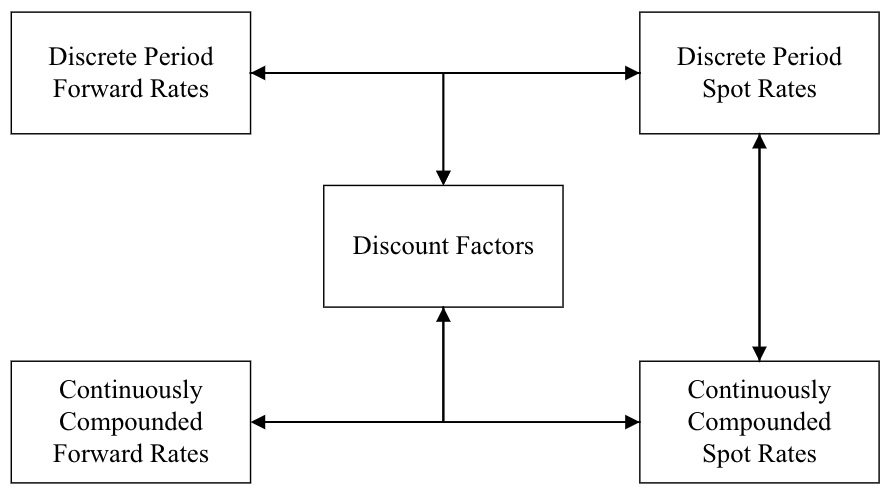
\includegraphics[width=0.9\textwidth]{Chapter_2/images/ch2_links.png}
\caption[Links between forward rates, spot rates, and discount factors]{A graphical representation of the links between different rates.}
\label{fig:linked_rates}
\end{center}
\end{figure}

The definitions and formulae presented in this section are critical to the understanding and subsequent pricing of interest rate derivatives. To fully appreciate their use, the reader is referred to Appendix \ref{append_A1} and \ref{append_A2} which contains detailed numerical examples. 